The input layer plays an important part in executing the spray painting task as per the programmed movement. The input in this system comes from the host PC and the sensors. The host PC acts as a centralized location to write programs for robotic movement, as well as control PLC logic. The sensors involved in the system are emergency stops (e-stops) and inductive switches. These inputs send signals to the PLC on particular situations and scenarios to keep the safety measure intact. Inductive switches make sure that the robot arm is calibrated properly before it executes its task. Where as emergency stops immediately halt the robot's operation, ensuring the safety of personnel and preventing potential accidents.


\subsection{Layer Hardware}
The sensors, including e-stops and inductive switches are the layer hardware for the input layer. 
%The sensors, including the vision sensor, e-stops, and gate, are connected to the programmable logical controller (PLC) via wires. They continuously transmit input values to the PLC, enabling the system to make informed decisions about subsequent actions.

\subsection{Layer Operating System}
Operating system used for this is Windows 10.
%RT ToolBox 3 Pro can be installed on both Windows 11 and Windows 10 operating systems.

\subsection{Layer Software Dependencies}
RT Toolbox is required.
%RT ToolBox 3, which controls the robot, will be used to facilitate the movement of the robot arm.

\subsection{E-Stops}
There will be multiple emergency stop (E-stop) buttons strategically placed throughout the system. These buttons will be located next to the case gate, on the controller, and inside the cage. When any of these e-stop buttons are pressed, the entire system will immediately halt, ensuring rapid response to any safety concerns or emergencies.


\begin{figure}[h!]
	\centering
 	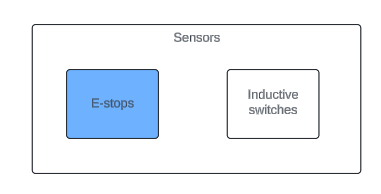
\includegraphics[width=0.60\textwidth]{images/E_stop_sensor.png}
 \caption{Sensor subsystem diagram}
\end{figure}

\subsubsection{Subsystem Hardware}
2 wired emergency stops connected to the CNUSR11 connector of the controller. 1 emergency stop located on the controller.

\subsubsection{Subsystem Operating System}
N/A

\subsubsection{Subsystem Software Dependencies}
N/A

\subsubsection{Subsystem Programming Languages}
N/A

\subsubsection{Subsystem Data Structures}
N/A

\subsubsection{Subsystem Data Processing}
The signals are send through wires to robot controller for processing to halt the robot.

\subsection{Inductive Switches}
Inductive switches are placed on the edges of linear rail to mark the endpoints. Using these switches will help the robot to calibrate the center of linear rail whenever robot starts.

\begin{figure}[h!]
	\centering
 	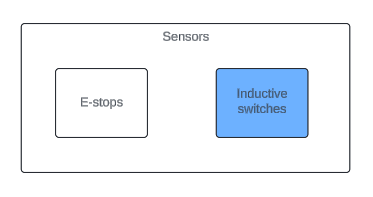
\includegraphics[width=0.60\textwidth]{images/Inductive_sensors.png}
 \caption{Sensors subsystem diagram}
\end{figure}

\subsubsection{Subsystem Hardware}
The inductive proximity sensor is a barrel-type sensor with PNP output, featuring a 1.5mm sensing range. It operates with a 3-wire configuration and is rated IP67. These sensors are typically connected to the general-purpose input/output pins of the PLC.%Inductive Proximity Sensors are used to limit the range of movement of the robot arm along the X-axis, E-stop sensors are utilized for emergency situations (True/False), and wires are employed to connect them to the PLC.

\subsubsection{Subsystem Operating System}
Windows 10.

\subsubsection{Subsystem Software Dependencies}
GX Works is needed in order to write ladder logic that processes the signals to act appropriately.

\subsubsection{Subsystem Programming Languages}
MELFA-BASIC VI programming language.

\subsubsection{Subsystem Data Structures}
N/A

\subsubsection{Subsystem Data Processing}
The switch sends a signal to the PLC when the robot passes over it. 

\subsection{RT Toolbox}
The RT Toolbox is a software package developed by Mitsubishi Electric for their industrial robots. It serves as a comprehensive toolset to assist with various tasks related to robot programming, configuration, and maintenance

\begin{figure}[h!]
	\centering
 	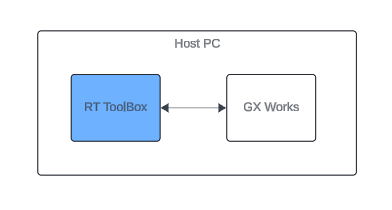
\includegraphics[width=0.60\textwidth]{images/RT_toolbox_Host.png}
 \caption{Host PC subsystem diagram}
\end{figure}

\subsubsection{Subsystem Hardware}
Host PC acts as system hardware in which RT Toolbox operates.

\subsubsection{Subsystem Operating System}
Windows 10.

\subsubsection{Subsystem Software Dependencies}
N/A

\subsubsection{Subsystem Programming Languages}
MELFA BASIC VI.

\subsubsection{Subsystem Data Structures}
Synchronous execution of the code.

\subsubsection{Subsystem Data Processing}
Utilizing Host PC's memory.

\subsection{GX Works}
GX Works3 is the configuration software for FX, L, and Q Series controllers developed by Mitsubishi Electric. GX Works3  interfaces with the work cell's programmable logic controller to program in several languages like ladder logic.

\begin{figure}[h!]
	\centering
 	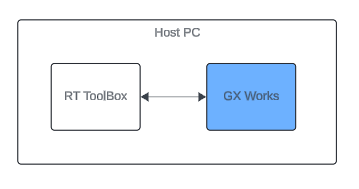
\includegraphics[width=0.60\textwidth]{images/GX_Works_Host.png}
 \caption{Host PC subsystem diagram}
\end{figure}

\subsubsection{Subsystem Hardware}
Host PC acts as system hardware.

\subsubsection{Subsystem Operating System}
Windows.

\subsubsection{Subsystem Software Dependencies}
N/A

\subsubsection{Subsystem Programming Languages}
Ladder Diagram (LD): A graphical representation of relay logic. \\
Structured Text (ST): A high-level textual language based on Pascal. \\
Function Block Diagram (FBD): A graphical language using function blocks. \\
Instruction List (IL): A low-level textual language. \\
Sequential Function Chart (SFC): A graphical language for sequential control.

\subsubsection{Subsystem Data Structures}
N/A

\subsubsection{Subsystem Data Processing}
Using Host PC's memory.